\subsection{\Acl{bflu} and \acl{mem}}\label{sec_fl_mem}

In this Section, we will build on the analysis of \cref{sec_fl_elastic}, and complexify the structure of the \acl{ela} with which \ac{bflu} interacts by considering, instead of an elastic material, an \ac{mem} \cite{helfrichElasticPropertiesLipid1973,derenyiFormationInteractionMembrane2002}.

For this problem, we will consider the  geometry depicted in \cref{fig_ref_cur_mem}. A vertical channel with mirror symmetry about its mid axis is considered. The left boundary of the channel is \pomin{}, and the right boundary \pomout{} lies on the symmetry axis. Fluid is injected from bottom to top on \pombottom. Here, \ac{mem} lies on the top boundary of \ac{bflu}, \pomtop{}, which  coincides with the \ac{mem} manifold \pomline{}. Finally, we denote by $\om$ the region enclosed by the boundaries, and all the quantities above will be considered in the \ac{ref} and \ac{cur} configurations.

The geometry of \cref{fig_ref_cur_mem} may represent \ac{bflu} being confined in a large reservoir, lying on bottom of the channel, where the channel is a vertical neck of the reservoir, covered on top by \ac{mem}.

\subsubsection{\Acl{mem} motion}
\label{sec_fl_mem_mem}

Both the physical nature and mathematical description of \ac{mem} is significantly more complex than that of \ac{ela}. First, unlike \ac{ela}, \ac{mem} has a fluid structure: its material elements can flow both tangentially and normally to it.
Such fluid behavior requires an Eulerian description, which then needs to be connected to the Lagrangian description used to describe \ac{dom}. Second, \ac{mem} is described by fourth-order \acp{pde} \cite{zhong-canBendingEnergyVesicle1989}, which are significantly more complex than the second-order \acp{pde} which describe \ac{ela} \cite{worthmullerIRENEFluIdLayeR2025}. Third, the geometrical description of \ac{mem} requires fixing an appropriate \textit{gauge}.
In fact, a general parametrization of \ac{mem} is given by two functions $\bxmemc(\xcoord^1)$. Both of these functions  depend on the curvilinear coordinate $\xcoord^1$ which is defined in the \ac{ref} domain of \ac{mem}, $\pomlineeqr$, see \cref{fig_ref_cur_mem}---note that here $\xcoord^i$ differs from the Cartesian coordinate $\xcartesian^\alpha$.
Despite this pair of functions, a single \ac{pde}  determines the \ac{mem} shape \cite{zhong-canBendingEnergyVesicle1989}.
To understand this redundancy, consider the  stretching field $\nu>0$, defined by
\begin{align}\label{eq_intro_nu}
    \nu ^ 2   & \equiv \bevec{1}   \cdot \bevec{1}, \\
    \label{eq_def_e}
    \bevec{i} & \equiv \pder{{\bxmemc}}{\xcoord^i}.
\end{align}
It is then easy to realize that two  parametrizations with different $\nu$s
may yield the same physical shape. Such  redundancy  may be removed by a gauge fixing, i.e., by adding a constraint on $\bxmemc$, or its derivatives.
Two common gauge choices are the Monge  \cite{hsiungFirstCourseDifferential1981,desernoFluidLipidMembranes2015}, or the arc-length parametrization \cite{derenyiFormationInteractionMembrane2002}, in which one sets
\be
\label{eq_arc_length_gauge}
\nu = 1.
\ee
The arc-length gauge has been used to describe, for instance, the steady state for membrane tubules \cite{derenyiFormationInteractionMembrane2002}. However, while a static constraint such as \crefs{eq_arc_length_gauge} is suited to  static shapes, it cannot describe the  \ac{mem} dynamics, such as the one of \ac{mem} interacting with \ac{bflu}. In fact, as \ac{mem} is deformed, it will also stretch: as a result, \cref{eq_arc_length_gauge} must be replaced by a time-dependent  gauge---see below.

We describe \ac{mem} with the Lagrangian approach, along the lines of the description of \ac{dom} in \cref{sec_fl_rigid} and \ac{ela}  in \cref{sec_fl_elastic}.  The \ac{mem} displacement field is
\be\label{eq_u_mem}
\bumem(\xcoord^1) \equiv \bxmemc(\xcoord^1) - \bxmemr(\xcoord^1),
\ee
where we choose the \ac{ref} configuration as a straight line
\be
\label{eq_def_x_ref}
\bxmemr(\xcoord^1) \equiv (\xcoord^1, h), \, 0 \leq  \xcoord^1 \leq L,
\ee
which is shown in \cref{fig_ref_cur_mem}A.
%
In addition, we introduce the  angle $\psi$ formed by the tangent to \ac{mem} with the $\xcartesian^1$ axis \cite{derenyiFormationInteractionMembrane2002}, defined by
\begin{align}
    \label{def_nu_psi_1}
    \evec{1}{1} & = \nu \cos \psi, \\
    \label{def_nu_psi_2}
    \evec{1}{2} & =-\nu \sin \psi.
\end{align}
Finally, the \ac{mem} metric tensor is defined by  \cite{marchiafavaAppuntiDiGeometria2005}
\be\label{eq_def_g}
g_{ij} \equiv \bevec{i} \cdot \bevec{j}.
\ee
In what follows, latin indices $i, j, k, \cdots$ will be used to denote vectors and tensors related to the \ac{mem} manifold; their position as upper and lower indexes is thus important \cite{marchiafavaAppuntiDiGeometria2005}. Because the differential manifold of \ac{mem} is one dimensional, indexes $i, j, k, \cdots$ may take only one value, i.e., $i=j=k= \cdots=1$. However, in formal relations such as \cref{eq_def_g}, we will use the general notation $i, j, k, \cdots$  for the sake of  generality, and for potential extensions of such relations to two-dimensional manifolds \cite{desernoFluidLipidMembranes2015}.
\vspace{0.5cm}\\


In order to work out the  dynamical equations for \ac{mem}, let us derive the force exerted by \ac{bflu} on \ac{mem}. The force exerted on a line element $\dint{l_\current}$ of \ac{mem}  is \cite{landauFluidMechanics1987}
\be
\label{def_f_fluid_mem}
f_{\fluid\, \alpha}(\sigmastressc, \nu, \psi) = - \sigmastressc_{\alpha \beta} \normalc{\gamma}(\nu, \psi),
\ee
where
\be
\label{eq_strees_tensor_fluid}
\sigmastressc_{\alpha \beta } \equiv \sigmafc \delta_{\alpha \beta}+ \eta_\fluid\left( \pderc{ \vfc^\alpha}{\beta} +\pderc{ \vfc^\beta}{\alpha}\right)
\ee
is the \ac{bflu} stress tensor \cite{landauFluidMechanics1987} and $\normalc{}$ the unit normal to $\pomtopeqc$ pointing outside $\omc$, see \cref{fig_ref_cur_mem}.  In \cref{def_f_fluid_mem}, $\sigmastressc$ is evaluated at the \ac{cur} coordinate $\bxmemc \in \pomtopeqc$ corresponding to $\xcoord^1$.
%
The components of the force \crefs{def_f_fluid_mem} tangential and normal to \ac{mem} are \cite{desernoFluidLipidMembranes2015}
\begin{align}
    \label{def_force_tan}
    f_{\fluid\, \text{t}}^i(\sigmastressc, \nu, \psi) & = g^{ij}(\nu) \evec{j}{\alpha}(\nu,\psi) f_\alpha(\sigmastressc, \nu, \psi) \\
    \label{def_force_norm}
    f_{\fluid\, \text{n}} (\sigmastressc, \nu, \psi)  & = \normalc{\alpha}(\nu, \psi) f_\alpha(\sigmastressc, \nu, \psi),
\end{align}
where in \cref{def_force_tan} we used the feature that the metric tensor depends on $\nu$ only, see \cref{eq_def_g,eq_intro_nu}.

The equations of motion for \ac{mem}  are \cite{worthmullerIRENEFluIdLayeR2025,al-izziShearDrivenInstabilitiesMembrane2020,arroyoRelaxationDynamicsFluid2009i}

\bw
\begin{align}
    \label{eq-dyn-continuity}
    \nab_i \vmem^i - 2 H \wmem                                                                              =            & 0,                                                                                                                                                                                                     \\
    \label{eq-dyn-v}
    \rhom \left( \pder{\vmem^i}{t}+ \vmem^j \nab_j \vmem^i  - 2 \vmem^j \wmem\, b^i_j - \wmem \nab^i \wmem \right)     = & \nab^i \sigmam + f_{\etam\, \text{t}}^i + f_{\fluid\, \text{t}}^i,                                                                                                                                     \\
    \label{eq-dyn-w}
    \rhom \left[ \pder{\wmem}{t} + \vmem^i ( \vmem^j b_{ji} + \nabla_i \wmem  ) \right]                               =  & 2 \sigmam H    +  f_\kap +                                                         f_{\etam\, \text{n}}+ f_{\fluid\, \text{n}}                                                                       , \\
    \label{eq-dyn-dX}
    \pder {\bumem}{t}                                                                                            =       & \wmem \normalc{},                                                                                                                                                                                      \\
    \label{eq-dyn-dX1}
    \pder {\umem^1}{x^1}                                                                                            =    & -1 + \nu \cos \psi,                                                                                                                                                                                    \\
    \label{eq-dyn-dX2}
    \pder {\umem^2}{x^1}                                                                                               = & -\nu \sin \psi,
\end{align}
\ew
and they hold for $\xcoord^1 \in \omlineeqr$.
%
Here, $\vmem^i$ and $w$ are the \ac{mem} tangential and normal velocity, respectively, $\nab$ is the covariant derivative related to the Levi-Civita connection associated to $g$, $\nablb$ the Laplace-Beltrami operator, $b$ the second fundamental form, and $H$ and $K$  the mean and Gaussian curvature, respectively.
We refer to \cite{desernoFluidLipidMembranes2015,worthmullerIRENEFluIdLayeR2025,marchiafavaAppuntiDiGeometria2005,arroyoRelaxationDynamicsFluid2009i} for details on the differential-geometry formulation, and we will now discuss each line in \cref{eq-dyn-continuity,eq-dyn-v,eq-dyn-w,eq-dyn-dX,eq-dyn-dX1,eq-dyn-dX2}.
\Cref{eq-dyn-continuity} enforces mass conservation \cite{landauFluidMechanics1987}.
\Cref{eq-dyn-v,eq-dyn-w} are the tangential and normal components of the \ac{ns} equations, respectively.
The first term in the \ac{rhs} of \cref{eq-dyn-v} represnts the force on membrane elements induced by gradients of line tension, while the first term in the \ac{rhs} of \cref{eq-dyn-w} constitutes Laplace pressure \cite{degennesCapillarityWettingPhenomena2004,landauFluidMechanics1987}. The other terms read
\begin{align}
    \label{eq_def_f_kap}
    f_\kap (\nu, \psi)                                                                                                       & \equiv                                                                                                  \newlinenn
    -2\kap [ \nab_i \nab^i H + 2 H (H^2-K)],                                                                                 &                                                                                                                                 \\
    \label{eq_def_f_eta_t}
    f_{\etam\, \text{t}}^i(\vmem, \wmem,
    \nu, \psi)                                                                                                               & \equiv                                                                                                             & \newlinenn
    \etam [ - \nablb \vmem^i - \newlinenn
    2 \left( b^{ij} - 2 \, H \, g^{ij}  \right) \nab_j \wmem + 2 K \vmem^i  ]                                                & ,                                                                                                                  &            \\
    \label{eq_def_f_eta_n}
    f_{\etam\, \text{n}}      (\vmem, \wmem, \nu, \psi)                                                                      & \equiv                                                                                                             & \newlinenn
    2 \etam [ (\nab^i \vmem^j)b_{ij} - 2 \wmem (2 H^2 - K)                                                                 ] & .
\end{align}
In \cref{eq_def_f_kap}, $f_\kappa$ is represents the resistance of \ac{mem} to bending, and it is derived from Helfrich model \cite{helfrichElasticPropertiesLipid1973}, while $f_{\etam\, t}$ and $f_{\etam\, \text{n}}$ in \cref{eq_def_f_eta_t,eq_def_f_eta_n} are, respectively, the tangential and normal component of the viscous force resulting from in-membrane flows \cite{arroyoRelaxationDynamicsFluid2009i}.
%
\Cref{eq-dyn-dX} is the time-evolution equation for the \ac{mem} shape, which evolves according to the normal $\normalc{}$, and it has been obtained from  \cref{eq_u_mem,eq_def_x_ref}.
\Cref{eq-dyn-dX1,eq-dyn-dX2} re-express the definitions of $\nu$ and $\psi$, and they result from \cref{def_nu_psi_1,def_nu_psi_2,eq_def_e,eq_u_mem,eq_def_x_ref}.
Finally, $\rhom$, $\sigmam$ and $\kappa$ are, respectively, the density, line tension and bending rigidity of \ac{mem}.



We choose the following \acp{bc} for \cref{eq-dyn-continuity,eq-dyn-v,eq-dyn-w,eq-dyn-dX,eq-dyn-dX1,eq-dyn-dX2}:
\begin{align}
    \label{bc_fl_mem_mem_1}
    \vmem^i                   & = 0 \text{ on } \pomlineineqr,        \\
    \label{bc_fl_mem_mem_2}
    \vmem^i                   & = 0 \text{ on } \pomlineouteqr,       \\
    \label{bc_fl_mem_mem_3}
    \wmem                     & = 0 \text{ on } \pomlineineqr,        \\
    \label{bc_fl_mem_mem_4}
    \nab_i \wmem              & = 0 \text{ on } \pomlineouteqr,       \\
    \label{bc_fl_mem_mem_5}
    \sigmam                   & = \sigmaml \text{ on } \pomlineineqr, \\
    \label{bc_fl_mem_mem_6}
    \bumem                    & = 0 \text{ on } \pomlineineqr,        \\
    \label{bc_fl_mem_mem_7}
    \umem^1                   & = 0 \text{ on } \pomlineouteqr,       \\
    \label{bc_fl_mem_mem_8}
    \pder{\umem^2}{\xcoord^1} & = 0 \text{ on } \pomlineouteqr.
\end{align}

\Cref{bc_fl_mem_mem_1,bc_fl_mem_mem_3,bc_fl_mem_mem_6} enforce the condition that the left extremity of \ac{mem}, \pomlinein, is clamped on the channel wall \pomin.
%
\Cref{bc_fl_mem_mem_4,bc_fl_mem_mem_7,bc_fl_mem_mem_8,bc_fl_mem_mem_2} enforce the mirror symmetry about \pomout.
Namely, \cref{bc_fl_mem_mem_2} ensures that the $\vmem$ vector field vanishes on \pomlineout, because a nonzero value of this field on \pomout{}  would break the axial symmetry. The condition \crefs{bc_fl_mem_mem_7} follows the same lines. In addition, the  symmetry requires that scalar fields and vertical components of vector fields in $\om$ have zero slope with respect to $\xcoord^1$ at \pomlineout{}, see \cref{bc_fl_mem_mem_4,bc_fl_mem_mem_8}.
Finally, \cref{bc_fl_mem_mem_5} fixes the \ac{mem} tension on \pomlinein.



\subsubsection{\Acl{dom} motion}
\label{sec_fl_mem_dom}



We will determine $\budom$ as the solution of a \ac{bvp} given by the following elastic model \cite{kamenskyLectureNotesMAE,marsdenMathematicalFoundationsElasticity1994}
\be\label{eq_mesh_fluid_rigid}
\pder{\Sdom_{\alpha \beta}(\budom)}{\xr^\beta} = 0 \text{ in } \omr,
\ee
where the elastic stress tensor $\Sdom$ is given by
\be
\label{eq_def_S}
\Sdom_{\alpha \beta} \equiv F_{\alpha \gamma} T_{\gamma \beta},
\ee
and
\begin{align}
    \label{eq_ela_1}
    T_{\alpha \beta}  \equiv & \kel(\budom) E_{\gamma \gamma} \delta_{\alpha \beta} +\newlinenn
                             & 2 \muel(\budom) \left(E_{\alpha \beta} - \frac{1}{2} \delta_{\alpha \beta} E_{\gamma \gamma}\right), \\
    \label{eq_ela_2}
    E_{\alpha \beta}  \equiv & \frac{1}{2}\left( F_{\gamma \alpha}F_{\gamma \beta} - \delta_{\alpha \beta}\right),                  \\
    \label{eq_ela_3}
    \kel(\bu)         \equiv & \frac{1}{[\det(F(\bu))]^\zeta},                                                                      \\
    \label{eq_ela_4}
    \muel(\bu)        \equiv & \frac{1}{[\det(F(\bu))]^\zeta}.
\end{align}
In \cref{eq_ela_3,eq_ela_4}, we included an additional dependence of bulk modulus $\kel$ and the shear modulus $\muel$ on the deformation-gradient tensor \crefs{eq_def_F}. In the absence of this dependence, the elastic model above would be unstable under local compression \cite{kamenskyLectureNotesMAE}. In fact, the model's Lagrangian would not penalize configurations with  small $\det F$. The inclusion of the dependence \crefs{eq_ela_3,eq_ela_4} on $\det F$  allows for penalizing these configurations---the larger the exponent $\zeta > 0$, the stronger the penalty. As a result, this dependence makes the model stable under mesh compression, such as the one shown below \ac{rig} in \cref{fig_ref_curr_rigid}B.

The equation of motion for $\budomdot$ is obtained by deriving \cref{eq_mesh_fluid_rigid} with respect to time, and using the fact that \ac{ref} coordinates are time independent:
\be
\label{eq_mesh_fluid_rigid_dot}
\pder{}{\xr^\beta}\der{\Sdom_{\alpha \beta}(\budom)}{t}  = 0 \text{ in } \omr.
\ee
We impose the following \acp{bc} for  \cref{eq_mesh_fluid_rigid,eq_mesh_fluid_rigid_dot}:
\begin{align}
    \label{bc_fl_mem_dom_1}
    \budom                   & = \bzero \text{ on }\pomineqr \cup \pombottomeqr, \\
    \label{bc_fl_mem_dom_2}
    \udom^1                  & = 0 \text{ on } \pomouteqr,                       \\
    \label{bc_fl_mem_dom_3}
    \pder{\udom^2}{\xr^1}    & = 0 \text{ on }\pomouteqr,                        \\
    \label{bc_fl_mem_dom_4}
    \budom                   & = \bumem \text{ on }\pomtopeqr,                   \\
    \label{bc_fl_mem_dom_5}
    \budomdot                & = \bzero \text{ on }\pomineqr \cup \pombottomeqr, \\
    \label{bc_fl_mem_dom_6}
    \udomdot^1               & = 0 \text{ on } \pomouteqr,                       \\
    \label{bc_fl_mem_dom_7}
    \pder{\udomdot^2}{\xr^1} & = 0 \text{ on }\pomouteqr,                        \\
    \label{bc_fl_mem_dom_8}
    \budomdot                & = \bumemdot \text{ on }\pomtopeqr.
\end{align}
\Cref{bc_fl_mem_dom_1} ensures that \ac{dom} is not deformed on $\pomineqr \cup \pombottomeqr$, cf. \cref{bc_ela_1}. \Cref{bc_fl_mem_dom_2,bc_fl_mem_dom_3} follow from axial symmetry, and \cref{bc_fl_mem_dom_4} from the requirement that \ac{dom} and \ac{mem} deformations stay conforming \cite{kamenskyLectureNotesMAE}. Finally, the  \acp{bc} for $\bumemdot$, \cref{bc_fl_mem_dom_5,bc_fl_mem_dom_6,bc_fl_mem_dom_7,bc_fl_mem_dom_8}, are derived along the same lines as \cref{bc_fl_mem_dom_1,bc_fl_mem_dom_2,bc_fl_mem_dom_3,bc_fl_mem_dom_4}.

We observe that \cref{eq_def_S,eq_ela_1,eq_ela_2,eq_ela_3,eq_ela_4} imply that \cref{eq_mesh_fluid_rigid,eq_mesh_fluid_rigid_dot} contains up to second derivatives of $\budom$ and $\budomdot$. As a result, the \acp{bc} \crefs{bc_fl_mem_dom_1,bc_fl_mem_dom_2,bc_fl_mem_dom_3,bc_fl_mem_dom_4,bc_fl_mem_dom_5,bc_fl_mem_dom_6,bc_fl_mem_dom_7,bc_fl_mem_dom_8} uniquely determine the solution of the \ac{bvp} \crefs{eq_mesh_fluid_rigid,eq_mesh_fluid_rigid_dot} \cite{evansPartialDifferentialEquations2010}.

\begin{figure}
    \centering
    \includegraphics[width=\columnwidth]{figures/figure_9/figure_9.pdf}
    \caption{
        \label{fig_ref_cur_mem}
        \Acl{ref} and \acl{cur} configuration for the interaction between a  \acf{bflu} and a \acf{mem}.
        The Figure follows the same notation as \cref{fig_ref_curr_rigid}, and it represents a vertical channel with mirror symmetry about its mid axis, which coincides with \pomout; the right, mirrored part of the channel is not shown.
        The top edge of the \ac{bflu} mesh, $\pomtopeqr$, coincides with the one-dimensional  manifold $\omlineeqr$ of \ac{mem}.
    }
\end{figure}

\begin{figure*}
    \centering
    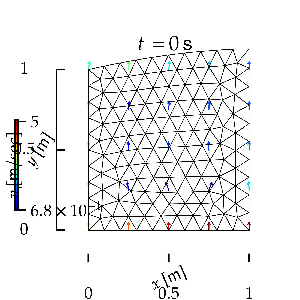
\includegraphics[width=\textwidth]{figures/figure_5/figure_5.pdf}
    \caption{
        Interaction between a \acf{bflu}  and a \acf{mem}. Here, \ac{bflu} is air, and \ac{mem} an elastomer, and the \ac{bflu} Reynolds number is $R \sim 200$.
        \plab{A}  \Acf{ref} and \acf{cur} configuration of \ac{mem} (red and green curve, respectively), and \ac{mem} displacement field $\bumem$ (black arrows).
        \plab{B} Stretch field of \ac{mem}.
        \plab{C} Tangent angle of \ac{mem}.
        \plab{D} and \plab{E}: \ac{bflu} velocity and tension, respectively; the notation is the same as in \cref{fig_fluid_rigid}.
        \plab{F}, \plab{G} and \plab{H}: Tangential velocity, normal velocity and tension of \ac{mem}, respectively.
        All panels refer to the same instant of time, shown on top, and they display also the deformed mesh (gray lines).
        \label{fig_fluid_mem}
    }
\end{figure*}

\subsubsection{\Acl{bflu} motion}
\label{sec_fl_mem_flu}

We will now discuss the \ac{bflu} equations of motion, and present them first in \ac{cur} configuration coordinates, and then transform them in \ac{ref} coordinates.


\paragraph{Equations of motion in  \acl{cur} configuration coordinates}
\label{sec_fl_mem_flu_cur}

In \ac{cur} coordinates, the \ac{bflu} equations of motion are the \ac{ns} and continuity equations \cite{landauFluidMechanics1987}:

\begin{align}
    \label{eq_fl_rigid_fl_1_current}
    \rho_\fluid \left( \partial_t \vfc^\alpha + \vfc^\beta  \pderc{\vfc^\alpha}{\beta} \right) & =  \pderc{  \sigmastressc_{\alpha \beta }}{\beta} ,                                              \\
    \label{eq_fl_rigid_fl_2_current}
    \pderc{ \vfc^\alpha }{\alpha}                                                              & =                                                              0                               ,
\end{align}
and they hold for $\bxc \in \omc$.
\Cref{eq_fl_rigid_fl_1_current,eq_fl_rigid_fl_2_current} describe the \ac{bflu} motion in a flat, two-dimensional geometry \cite{landauFluidMechanics1987}---an example of the corresponding  \ac{ns} equations on a curved geometry is given by \cref{eq-dyn-v}.




We enforce the following \acp{bc} for \cref{eq_fl_rigid_fl_1_current,eq_fl_rigid_fl_2_current}:
\begin{align}
    \label{bc_fl_membrane_1_current}
    \bvfc             & =  \vfbottom  \text{ on } \pombottomeqc,                                                                 \\
    \label{bc_fl_membrane_2_current}
    \bvfc             & =  \bzero  \text{ on } \pomineqc,                                                                        \\
    \label{bc_fl_membrane_3_current}
    \vfc^1            & =  0 \; \text{ on } \pomouteqc ,                                                                         \\
    \label{bc_fl_membrane_4_current}
    \pderc{\vfc^2}{2} & =  0 \; \text{ on } \pomouteqc ,                                                                         \\
    \label{bc_fl_membrane_5_current}
    \bvfc(\bxc)       & = \left. \der{\bumem(\xcoord^1)}{t} \right|_{\xcoord^1 = [{\bm \psi}^t(\bxc)]^1} \text{ on } \pomtopeqc, \\
    \label{bc_fl_membrane_6_current}
    \sigmafc          & = \sigmafbottomc \text{ on } \pombottomeqc.
\end{align}

According to \cref{bc_fl_membrane_1_current}, \ac{bflu} is injected from the bottom edge of $\omc$, \pombottomc, while \cref{bc_fl_membrane_2_current} is a no-slip \ac{bc} on the left wall \pominc, and \cref{bc_fl_membrane_3_current,bc_fl_membrane_4_current} result from symmetry.
\Cref{bc_fl_membrane_5_current} ensures that the motion of \ac{bflu} is conforming to that of \ac{mem}   \cite{kamenskyLectureNotesMAE}: In fact,   \cref{eq-dyn-dX} ensures that \ac{mem}  only moves normally to its profile, and \cref{bc_fl_membrane_5_current} thus ensures that \ac{bflu} stays in contact with \ac{mem} throughout its motion. On the other hand, \cref{bc_fl_membrane_5_current} implies a tangential slip between \ac{mem} and \ac{bflu}, allowing for the tangential part of the \ac{bflu} and \ac{mem} velocities to differ.
Finally,  \cref{bc_fl_membrane_6_current} stems from the presence of the reservoir, in which the \ac{bflu}  tension is equal to $\sigmafbottomc$: At the boundary $\pombottomeqc$ between the channel and the reservoir, the \ac{bflu} tension  matches the reservoir's.


\paragraph{Equations of motion in  \acl{ref} configuration coordinates}
\label{sec_fl_mem_flu_ref}

We will now rewrite the equations of motion and the \acp{bc} of \cref{sec_fl_mem_flu_cur} in terms of $\bvfr$, $\sigmafr$, and the \ac{ref} coordinate $\bxr$. The equations of motion \crefs{eq_fl_rigid_fl_1_current,eq_fl_rigid_fl_2_current} yield, respectively,
\bw
\begin{align}
    \label{eq_fl_rigid_fl_1_reference}
    \rhof \left\{ \pder{ \vfr^\alpha(\bxr, t)}{t} + \left[ \vfr^\gamma(\bxr, t)  - \der{\varphi^{\gamma\, t}(\bxr)}{t}\right]  G_{\beta \gamma}(\budom^t(\bxr)) \frac{\partial  \vfr^\alpha(\bxr, t)}{\partial \xr^\beta} \right\}                                                       & =              \newlinenn
    G_{\beta \alpha}(\budom^t(\bxr))  \,          \pderr{ \sigmafr(\bxr, t)   }{\beta }                + \etaf \,              G_{\delta \beta}(\budom^t(\bxr))           \,         \pderr{}{\delta} \left[  G_{\gamma \beta}(\budom^t(\bxr)) \pderr{ \vfr(\bxr, t)}{\gamma}   \right], &                           \\
    \label{eq_fl_rigid_fl_2_reference}
    G_{\beta \alpha}(\budom^t(\bxr)) \pderr{ \vfr^\alpha(\bxr, t)}{\beta}                                                                                                                                                                                                                & = 0,
\end{align}
\ew
which hold in $\omr$. In \cref{eq_fl_rigid_fl_1_reference,eq_fl_rigid_fl_2_reference} the tensor $G$ is given by the inverse of $F$ \cite{kamenskyLectureNotesMAE}:
\be
\label{eq_def_G}
G_{\alpha \beta}(\bu) \equiv [F(\bu)]^{-1}_{\alpha \beta}.
\ee\vspace{5mm}\\



\subsubsection{Temporal discretization}\label{sec_temp_discretization_mem}

To numerically solve for the dynamics in a time span $0 \leq t \leq T$, we discretize time by setting $\deltat \equiv T/N$, $t_n \equiv n\, \deltat$, with $n = 0, 1, \cdots, N$.

We combine the \ac{cn} discretization method for \ac{ns} equations \cite{loggAutomatedSolutionDifferential2012,crankPracticalMethodNumerical1947} with the \ac{ale} formulation, by discretizing the dynamical equations for \ac{mem}, \ac{dom} and \ac{bflu}.
The  dynamics of the system is obtained as follows.\\ \vspace{5mm}


Following the \ac{cn} temporal-discretization scheme \cite{crankPracticalMethodNumerical1947}, we define fields at staggered,  integer and semi-integer time steps  \cite{loggAutomatedSolutionDifferential2012}: For example, we set
\begin{align}
    \label{eq_time_step_1}
    \bvfr^n(\bxr)          & \equiv \bvfr(\bxr, t_n)  ,                               \\
    \label{eq_time_step_2}
    \sigmafr^{n-1/2}(\bxr) & \equiv \sigmafr\left(\bxr, \frac{t_n+t_{n-1}}{2}\right),
\end{align}
and similarly for other \ac{bflu} and \ac{mem} fields.




%C add details in these sections - start 
\paragraph{\Acl{mem}}\label{sec_temp_discretization_mem_mem}


We discretize \cref{eq-dyn-v,eq-dyn-w,eq-dyn-continuity,eq-dyn-dX,eq-dyn-dX1,eq-dyn-dX2} as follows
\bw
\begin{align}
    \label{eq_mem_flu_disc_3}
    \nab^\nmhalf_i \vmem^i - 2 H^\nmhalf \wmem^n                                                                              =                                                                                                                                     & 0,                        \\
    \label{eq_mem_flu_disc_1}
    \rhom \Big(  \frac{\vmem^{n,\, i} - \vmem^{n-1,\, i}}{\deltat} +   \frac{3}{2}\vmem^{n-1,\, j}  \nab^{\nmhalf}_j \vmem^{n-1,\, i} -   \frac{1}{2}\vmem^{n-2,\, j}  \nab^{\nmhalf}_j \vmem^{n-2,\, i} - 2 \vmem^{n-1,\, j} \wmem^{n-1} \fnij{b}{\nmhalf}{i}{j} - & \newlinenn
    \wmem^{n-1} \nab^{\nmhalf, \, i} \wmem^{n-1} \Big)                                                                                                                                                                                                              & =              \newlinenn
    \nab^{\nmhalf, \, i} \sigmam^\nmhalf     +         f_{\etam\, \text{t}}^i\left( \frac{\bvmem^n + \bvmem^{n-1}}{2}, \frac{\wmem^n + \wmem^{n-1}}{2}, \nu^\nmhalf, \psi^\nmhalf\right) + \newlinenn
    f_{\fluid\, \text{t}}^i({\bm \sigmastressr}(\bvfr^{n-1}, \sigmafr^{n-3/2}, \budom^{n-1}), \nu^\nmhalf, \psi^\nmhalf) ,                                                                                                                                          &
    \\
    \label{eq_mem_flu_disc_2}
    \rhom \left( \frac{\wmem^n - \wmem^{n-1}}{\deltat} + \vmem^{n-1,\, i} \vmem^{n-1,\, j} b^\nmhalf_{ji} + \frac{3}{2} \vmem^{n-1, \, i}  \nab^\nmhalf_i \wmem^{n-1}  - \frac{1}{2} \vmem^{n-2, \, i}  \nab^\nmhalf_i \wmem^{n-2} \right)                          & =\newlinenn
    f_\kap(\nu^\nmhalf,\psi^\nmhalf) + 2 \sigmam^\nmhalf H^\nmhalf + f_{\etam\, \text{n}}     \left( \frac{\bvmem^n + \bvmem^{n-1}}{2}, \frac{\wmem^n + \wmem^{n-1}}{2}, \nu^\nmhalf, \psi^\nmhalf\right) + \newlinenn
    f_{\fluid\, \text{n}} ({\bm \sigmastressr}(\bvfr^{n-1}, \sigmafr^{n-3/2}, \budom^{n-1}), \nu^\nmhalf, \psi^\nmhalf),                                                                                                                                            &\end{align}
\ew
\begin{align}
    \label{eq_mem_flu_disc_4}
    \frac {\bumem^\nmhalf-\bumem^\nmthreehalf}{\deltat}                                                                                 = & \wmem^{n-1} \normalc{\nmhalf}, \\
    \label{eq_mem_flu_disc_5}
    \pder {\umem^{\nmhalf, \, 1}}{x^1}                                                                                            =       &
    -1 + \nu^\nmhalf \cos \psi^\nmhalf,                                                                                                                                    \\
    \label{eq_mem_flu_disc_6}
    \pder {\umem^{\nmhalf, \, 2}}{x^1}                                                                                               =    &
    -\nu^\nmhalf \sin \psi^\nmhalf.
\end{align}
In \cref{eq_mem_flu_disc_1,eq_mem_flu_disc_2}, $\sigmastressr$ denotes the \ac{bflu} stress tensor in the \ac{ref} configuration:
\begin{align}
    \label{eq_def_sigma_current}
    \sigmastressr^t_{\alpha \beta}(\bxr)  \equiv & \sigmastressc_{\alpha \beta}({\bm \varphi}^t(\bxr)) \newlinenn
    =                                            & \sigmafr(\bxr, t) \delta_{\alpha \beta} + \etaf \Big[ G_{\gamma \beta}(\budom^t(\bxr)) \pderr{\vfc^\alpha}{\gamma} + \newlinenn
                                                 & G_{\gamma \alpha}(\budom^t(\bxr)) \pderr{\vfc^\beta}{\gamma}\Big].
\end{align}

Proceeding along the same lines, the discrete form of the \acp{bc} \crefs{bc_fl_mem_mem_1,bc_fl_mem_mem_2,bc_fl_mem_mem_3,bc_fl_mem_mem_4,bc_fl_mem_mem_5,bc_fl_mem_mem_6,bc_fl_mem_mem_7,bc_fl_mem_mem_8} reads, respectively,
\begin{align}
    \label{bc_fl_mem_mem_1_disc_bis}
    \vmem^{n, \,i}                          & = 0 \text{ on } \pomlineineqr,        \\
    \label{bc_fl_mem_mem_2_disc_bis}
    \vmem^{n, \, i}                         & = 0 \text{ on } \pomlineouteqr,       \\
    \label{bc_fl_mem_mem_3_disc_bis}
    \wmem^n                                 & = 0 \text{ on } \pomlineineqr,        \\
    \label{bc_fl_mem_mem_4_disc_bis}
    \nab^\nmhalf_i \wmem^n                  & = 0 \text{ on } \pomlineouteqr,       \\
    \label{bc_fl_mem_mem_5_disc_bis}
    \sigmam^\nmhalf                         & = \sigmaml \text{ on } \pomlineineqr, \\
    \label{bc_fl_mem_mem_6_disc_bis}
    \bumem^\nmhalf                          & = 0 \text{ on } \pomlineineqr,        \\
    \label{bc_fl_mem_mem_7_disc_bis}
    \umem^{\nmhalf, \, 1}                   & = 0 \text{ on } \pomlineouteqr,       \\
    \label{bc_fl_mem_mem_8_disc_bis}
    \pder{\umem^{\nmhalf, \, 2}}{\xcoord^1} & = 0 \text{ on } \pomlineouteqr.
\end{align}

In what follows, we will split the \ac{bvp} into three steps \cite{loggAutomatedSolutionDifferential2012,chorinNumericalSolutionNavierStokes1968}:
\begin{enumerate}
    \titleditem{Approximated velocities}{
        \label{item_mem_split_1}
        Proceeding along the lines of the splitting scheme for  \ac{bflu} of \cref{sec_splitting_scheme_fl_rig_fl}, we introduce the auxiliary  velocities $\bvbarmem$ and $\wbarmem$, which approximate, respectively, $\bvmem^n$ and $\wmem^n$ \cite{chorinNumericalSolutionNavierStokes1968}. We define $\bvbarmem$ and $\wbarmem$ as solutions of the \acp{pde}
        \bw
        \begin{align}
            \label{eq_fl_mem_mem_disc_1}
            \rhom \Big[  \frac{\vbarmem^i - \vmem^{n-1,\, i}}{\deltat} +  \left( \frac{3}{2}\vmem^{n-1,\, j} - \frac{1}{2} \vmem^{n-2,\, j} \right)     \nab^{\nmhalf}_j \Vmem^i - 2 \Vmem^j \Wmem \fnij{b}{\nmhalf}{i}{j} -    \Wmem \nab^{\nmhalf, \, i} \Wmem \Big] & =              \newlinenn
            \nab^{\nmhalf, \, i} \sigmamast     +         f_{\etam, \text{t}}^i\left( \bVmem, \Wmem, \nu^\nmhalf, \psi^\nmhalf\right) + \newlinenn
            f_{\fluid\, \text{t}}^i({\bm \sigmafr}(\bvfr^{n-1}, \sigmafr^{n-3/2}, \budom^{n-1}), \nu^\nmhalf, \psi^\nmhalf) ,                                                                                                                                          &                           \\
            \label{eq_fl_mem_mem_disc_2}
            \rhom \left[ \frac{\wbarmem - \wmem^{n-1}}{\deltat} + \Vmem^i \Vmem^j b^\nmhalf_{ji} + \left( \frac{3}{2} \vmem^{n-1, \, i} - \frac{1}{2}\vmem^{n-3/2,\,i}\right) \nab^\nmhalf_i \Wmem \right]                                                             & =\newlinenn
            f_\kap(\nu^\nmhalf,\psi^\nmhalf) + 2 \sigmamast H^\nmhalf + f_{\etam\, \text{n}}      (\bVmem, \Wmem, \nu^\nmhalf, \psi^\nmhalf) + \newlinenn
            f_{\fluid\, \text{n}} ({\bm \sigmafr}(\bvfr^{n-1}, \sigmafr^{n-3/2}, \budom^{n-1}), \nu^\nmhalf, \psi^\nmhalf)                                                                                                                                             & ,
        \end{align}
        \ew
        where we have set
        \begin{align}
            \label{eq_def_Vmem}
            \Vmem^i    & \equiv \frac{\vbarmem^i + \vmem^{n-1,\,i}}{2}, \\
            \label{eq_def_Wmem}
            \Wmem      & \equiv \frac{\wbarmem + \wmem^{n-1}}{2},       \\
            \label{eq_def_sigmamasst}
            \sigmamast & \equiv \sigmam^{n-3/2},
        \end{align}
        \Cref{eq_fl_mem_mem_disc_1,eq_fl_mem_mem_disc_2} are the analog of \cref{eq_mem_flu_disc_1,eq_mem_flu_disc_2}, respectively,  with a fixed pressure field $\sigmamast$ from the preceding step---in what follows, we will synonymously use the terms `pressure' and `tension'  for conciseness \cite{worthmullerIRENEFluIdLayeR2025}.

        Overall, \cref{eq_fl_mem_mem_disc_1,eq_fl_mem_mem_disc_2} determine $\vbarmem$ and $\wbarmem$.
    }
    \titleditem{Pressure correction}{
        \label{item_mem_split_2}
        Subtracting \cref{eq_mem_flu_disc_1,eq_fl_mem_mem_disc_1} and neglecting $\odeltat$ \cite{worthmullerIRENEFluIdLayeR2025}, we obtain
        \be
        \label{eq_fl_mem_mem_disc_4}
        \rhom \frac{\vmem^{n, \, i} - \vbarmem^i }{\deltat}                         =   - \nab^{\nmhalf, \, i}\phimem,
        \ee
        where we have defined the pressure increment as
        \begin{align}
            \label{eq_def_phimem}
            \phimem & \equiv \sigmamast - \sigmam^\nmhalf.
        \end{align}
        Proceeding along the same lines for \cref{eq_mem_flu_disc_2,eq_fl_mem_mem_disc_2}, we obtain
        \be
        \label{eq_fl_mem_mem_disc_5}
        \wmem^n                                                                     =  \wbarmem.
        \ee
        By taking the covariant derivative of \cref{eq_fl_mem_mem_disc_4} and using the mass-conservation equation \crefs{eq_mem_flu_disc_3} and \cref{eq_fl_mem_mem_disc_5}, we obtain
        \begin{align}
            \label{eq_poisson_like_phi_mem}
            \nab^\nmhalf_i \nab^{\nmhalf,\, i} \phimem                                & =  \newlinenn
            \frac{\rhom}{\deltat} (\nab^\nmhalf_i \vbarmem^i - 2 H^\nmhalf \wbarmem). &
        \end{align}
        \Cref{eq_poisson_like_phi_mem} is a second-order \ac{pde} which determines $\phimem$, and thus the tension $\sigmam^\nmhalf$ through \cref{eq_def_phimem}.
    }
    \titleditem{Velocity correction}{
        \label{item_mem_split_3}
        The \ac{mem} velocity $\bvmem^n$ is determined by means of \cref{eq_poisson_like_phi_mem} in terms of $\bvbarmem$ and $\phimem$.
    }
\end{enumerate}

The \acp{bc} for \cref{eq_fl_mem_mem_disc_1,eq_fl_mem_mem_disc_2,eq_fl_mem_mem_disc_4,eq_fl_mem_mem_disc_5,eq_mem_flu_disc_4,eq_mem_flu_disc_5,eq_mem_flu_disc_6,eq_poisson_like_phi_mem} are
\begin{align}
    \label{bc_fl_mem_mem_1_disc}
    \vbarmem^i                                         & = 0 \text{ on } \pomlineineqr,  \\
    \label{bc_fl_mem_mem_2_disc}
    \vbarmem^i                                         & = 0 \text{ on } \pomlineouteqr, \\
    \label{bc_fl_mem_mem_3_disc}
    \wbarmem                                           & = 0 \text{ on } \pomlineineqr,  \\
    \label{bc_fl_mem_mem_4_disc}
    \nab^\nmhalf_i \wbarmem                            & = 0 \text{ on } \pomlineouteqr, \\
    \label{bc_fl_mem_mem_5_disc}
    \phimem                                            & = 0 \text{ on } \pomlineineqr,  \\
    \label{bc_fl_mem_mem_6_disc}
    \normalmem^\nmhalf_i  \nab^{\nmhalf, \, i} \phimem & = 0 \text{ on } \pomlineeqr,    \\
    \label{bc_fl_mem_mem_7_disc}
    \bumem^{\nmhalf}                                   & = 0 \text{ on } \pomlineineqr,  \\
    \label{bc_fl_mem_mem_8_disc}
    \umem^{\nmhalf,\, 1}                               & = 0 \text{ on } \pomlineouteqr, \\
    \label{bc_fl_mem_mem_9_disc}
    \pder{\umem^{\nmhalf, \, 2}}{x^1}                  & = 0 \text{ on } \pomlineouteqr.
\end{align}


In \cref{bc_fl_mem_mem_6_disc}, $\bm \normalmem$ is the unit normal to \pomline{}: It lies in the tangent bundle of $\omlineeq$, it is directed  outside $\omlineeq$, and it is normalized according to $\normalmem^i \normalmem_i = 1$ \cite{reallGeneralRelativity,marchiafavaAppuntiDiGeometria2005,worthmullerIRENEFluIdLayeR2025}.

\paragraph{\Acl{dom}}\label{sec_temp_discretization_mem_dom}

The discretization of the equations of motion for  \ac{dom} proceeds along the same lines as in \cref{sec_fl_rigid}, see \cref{sec_splitting_scheme_fl_rig_dom}. The discrete version of the \acp{pde} \crefs{eq_mesh_fluid_rigid,eq_mesh_fluid_rigid_dot} is

\begin{align}
    \label{eq_domain_fluid_rigid_disc}
    \pder{\Sdom_{\alpha \beta}(\budom^n)}{\xr^\beta}          & = 0 \text{ in } \omr, \\
    \label{eq_domain_fluid_rigid_disc_dot}
    \pder{}{\xr^\beta}\der{\Sdom_{\alpha \beta}(\budom^n)}{t} & = 0 \text{ in } \omr,
\end{align}
with \acp{bc} given by the discrete version of \cref{bc_fl_mem_dom_1,bc_fl_mem_dom_2,bc_fl_mem_dom_3,bc_fl_mem_dom_4,bc_fl_mem_dom_5,bc_fl_mem_dom_6,bc_fl_mem_dom_7,bc_fl_mem_dom_8}:
\begin{align}
    \label{bc_fl_mem_dom_1_disc}
    \budom^n                         & = \bzero \text{ on } \pomineqr \cup \pombottomeqr, \\
    \label{bc_fl_mem_dom_2_disc}
    \udom^{n, \, 1}                  & = 0 \text{ on } \pomouteqr,                        \\
    \label{bc_fl_mem_dom_3_disc}
    \pder{\udom^{n, \, 2}}{\xr^1}    & = 0 \text{ on } \pomouteqr,                        \\
    \label{bc_fl_mem_dom_4_disc}
    \budom^n                         & = \bumem^{\nmhalf} \text{ on } \pomtopeqr,         \\
    \label{bc_fl_mem_dom_5_disc}
    \budomdot^n                      & = \bzero \text{ on } \pomineqr \cup \pombottomeqr, \\
    \label{bc_fl_mem_dom_6_disc}
    \udomdot^{n, \, 1}               & = 0 \text{ on } \pomouteqr,                        \\
    \label{bc_fl_mem_dom_7_disc}
    \pder{\udomdot^{n, \, 2}}{\xr^1} & = 0 \text{ on } \pomouteqr,                        \\
    \label{bc_fl_mem_dom_8_disc}
    \budomdot^n                      & = \bumem^{\nmhalf} \text{ on } \pomtopeqr.
\end{align}



\paragraph{\Acl{bflu}}\label{sec_temp_discretization_mem_bflu}


The discretization of the equations of motion for  \ac{bflu} proceeds along the same lines as in \cref{sec_fl_rigid}, and is split into three steps: Approximated velocity, pressure correction and velocity correction, see \cref{sec_splitting_scheme_fl_rig_fl}.



The resulting \acp{pde} for $\bvbarf$ and $\sigmafr$ are
\bw
\begin{align}
    \label{eq_fl_rigid_fl_1_reference_disc_aux}
    \rhof \left\{  \frac{\vbarf^\alpha - \vfr^{n-1,\, \alpha}}{\deltat} + \left[ \frac{3}{2} ( \vfr^{n-1,\, \gamma}  -  \udomdot^{n-1,\, \gamma}) \, G_{\beta \gamma}(\budom^{n-1})  - \frac{1}{2} ( \vfr^{n-2,\, \gamma}  -  \udomdot^{n-2,\, \gamma}) \, G_{\beta \gamma}(\budom^{n-2})  \right] \frac{\partial  \Vf^\alpha}{\partial \xr^\beta}\right\} & =              \newlinenn
    G_{\beta \alpha}(\budom^{n-1})  \,          \pderr{ \sigmafr^\ast   }{\beta }                + \etaf \,              G_{\delta \beta}(\budom^{n-1})            \,         \pderr{}{\delta} \left(  G_{\gamma \beta}(\budom^{n-1}) \pderr{\Vf^\alpha }{\gamma}    \right),                                                                                                          \\
    \label{eq_poiss_like_phi}
    \frac{\rhof}{\deltat} G_{\gamma \alpha}(\budom^{n-1}) \pderr{\vbarf^\alpha }{\gamma}                                                                                                                                                                                                                                                                   & = \newlinenn
    G_{\gamma \alpha}(\budom^{n-1}) \pderr{}{\gamma}\left( G_{\beta \alpha}(\budom^{n-1})  \,          \pderr{ \phif   }{\beta } \right)                                                                                                                                                                                                                   & ,
\end{align}
\ew
where we have set
\begin{align}
    \label{eq_def_Vf}
    \bVf          & \equiv\frac{ \bvbarf + {\bm \vfr}^{n-1}}{2}, \\
    \label{eq_def_sigmarast}
    \sigmafr^\ast & \equiv \sigmafr^{n-3/2},                     \\
    \label{eq_def_phi_pressure}
    \phif         & \equiv \sigmafr^\ast - \sigmafr^{n-1/2}.
\end{align}


The \acp{bc} for \cref{eq_fl_rigid_fl_1_reference_disc_aux,eq_poiss_like_phi} are \cite{loggAutomatedSolutionDifferential2012}
\begin{align}
    \label{bc_fl_membrane_1_current_disc}
    \bvbarf                                         & =  \vfbottom  \text{ on } \pombottomeqr, \\
    \label{bc_fl_membrane_2_current_disc}
    \bvbarf                                         & =  \bzero  \text{ on } \pomineqr,        \\
    \label{bc_fl_membrane_3_current_disc}
    \vbarf^1                                        & =  0 \; \text{ on } \pomouteqr ,         \\
    \label{bc_fl_membrane_4_current_disc}
    G(\budom^{n-1})_{\alpha 1}\pderr{\Vf^2}{\alpha} & =  0 \; \text{ on } \pomouteqr ,
\end{align}
\begin{align}
    \label{bc_fl_membrane_5_current_disc}
    \bvbarf(x^1, h) & = \umemdot^\nmhalf(x^1)  \text{ on } \pomtopeqr, & \\
    \label{bc_fl_membrane_6_current_disc}
    \phif           & = 0 \text{ on } \pombottomeqr,
\end{align}
\begin{align}
    \label{bc_fl_membrane_7_current_disc}
    \normalr{\gamma}  G_{\gamma \alpha}(\budom^{n-1})  G_{\beta \alpha}(\budom^{n-1})
    \pderr{ \phif   }{\beta }                        & = \newlinenn
    0
    \text{ on } \pomineqr \cup \pomtopeqr ,          &                             \\
    \label{bc_fl_membrane_8_current_disc}
    G(\budom^{n-1})_{\alpha 1} \pderr{\phif}{\alpha} & = 0 \text{ on } \pomouteqr.
\end{align}


Finally, $\bvfr^n$ is determined from $\bvbarf $ and $\sigmafr^\nmhalf$ by means of the relation

\be
\label{eq_phi_1}
\rhof \frac{\vbarf^\alpha - \vfr^{n, \, \alpha}}{\deltat}  = G_{\beta \alpha}(\budom^{n-1})         \pderr{ \phif   }{\beta } \text{ in } \omr.
\ee\vspace{1cm}\\


%C add details in these sections - end



Given the \ac{mem} fields $\vmem^{n-1, i}$, $\wmem^{n-1, \, i}$, $\sigmam^{n-3/2}$, $\bumem^{n-3/2}$, $\nu^{n-3/2}$, $\psi^{n-3/2}$, the \ac{dom} fields $\budom^{n-1}$, $\budomdot^{n-1}$, and the \ac{bflu} fields $\bvfr^{n-1}$, $\sigmafr^{n-3/2}$, we determine the fields at the next time step $n \rightarrow n+1$ as follows:


\begin{itemize}
    \titleditem{Update \ac{mem}}{ \label{fl_mem_step_1}
        The \ac{mem} fields $\vmem^{n, i}$, $\wmem^{n, \, i}$, $\sigmam^{n-1/2}$, $\bumem^{n-1/2}$, $\nu^{n-1/2}$, $\psi^{n-1/2}$ are determined by solving the \ac{bvp} given by  \cref{eq_fl_mem_mem_disc_1,eq_fl_mem_mem_disc_2,eq_fl_mem_mem_disc_4,eq_fl_mem_mem_disc_5,eq_mem_flu_disc_4,eq_mem_flu_disc_5,eq_mem_flu_disc_6,eq_poisson_like_phi_mem,bc_fl_mem_mem_1_disc,bc_fl_mem_mem_2_disc,bc_fl_mem_mem_3_disc,bc_fl_mem_mem_4_disc,bc_fl_mem_mem_5_disc,bc_fl_mem_mem_6_disc,bc_fl_mem_mem_7_disc,bc_fl_mem_mem_8_disc,bc_fl_mem_mem_9_disc}.
    }

    \titleditem{Update \ac{dom}}{ \label{fl_mem_step_2}
        We determine the \ac{dom} displacement field and its time derivative, $\budom^n$ and $\budomdot^n$, from the \acp{bvp} given by \cref{eq_domain_fluid_rigid_disc,eq_domain_fluid_rigid_disc_dot,bc_fl_mem_dom_1_disc,bc_fl_mem_dom_2_disc,bc_fl_mem_dom_3_disc,bc_fl_mem_dom_4_disc,bc_fl_mem_dom_5_disc,bc_fl_mem_dom_6_disc,bc_fl_mem_dom_7_disc,bc_fl_mem_dom_8_disc}.

    }

    \titleditem{Update \ac{bflu}}{ \label{fl_mem_step_3}
        We determine the \ac{bflu} fields $\bvmem^n $ and $\sigmafr^\nmhalf$ by solving the \ac{bvp} given by  \cref{eq_fl_rigid_fl_1_reference_disc_aux,eq_poiss_like_phi,bc_fl_membrane_1_current_disc,bc_fl_membrane_2_current_disc,bc_fl_membrane_3_current_disc,bc_fl_membrane_4_current_disc,bc_fl_membrane_5_current_disc,bc_fl_membrane_6_current_disc,bc_fl_membrane_7_current_disc,bc_fl_membrane_8_current_disc}, and by solving  \cref{eq_phi_1}.

    }
\end{itemize}

The fields ${\bm \vfc}^n$, $\sigmafc^{n-1/2}$ in the \ac{cur} configuration are then obtained from the respective fields in the \ac{ref} configuration through \cref{eq_vf_ref,eq_sigmaf_ref}.\\ \vspace{5mm}


An example of this dynamics is shown in \cref{fig_fluid_mem}, where we show the interaction between air (\ac{bflu}) and an elastomer (\ac{mem}).
The  channel has dimensions $L = 1 \, \met$, $h = 0.2 \, \met$. Proceeding along the lines of \cref{sec_fl_rigid},   \ac{mem} parameters have been estimated by considering the parameters for a three-dimensional material, multiplying them by a unit length corresponding to the out-of-plane depth, and by the \ac{mem} thickness, chosen to be $\Delta = 10^{-3}\, \met$. The \ac{mem} bending rigidity $\kap$ has been estimated from the relation $\kap = E \Delta^3/[12(1-\nu^2)]$, which expresses $\kap$ as a function of the Young modulus $E$, the Poisson ratio $\nu$, and  $\Delta$ \cite{landauTheoryElasticity1986}. Typical values for an elastomer   are $E \sim 10^7 \, \pas$ \cite{fengPreparationCharacterizationSilicone2017} and $\nu \sim 0.5$ \cite{mullerQuickAccurateMethod2019}, yielding $\kap = 10^{-3} \, \kg \, \met^3/\sec^2$.
We chose $\rhom = 1 \, \kg /  \met$ and $\etam = 1 \, \kg\, \met /\sec $ as the density and viscosity of an elastomer, respectively \cite{caiSoftPolydimethylsiloxaneElastomers2015,pochivalovDevelopmentVibrationDamping2021},  and we take $\sigmaml = 1 \, \newt$.
The \ac{bflu} parameters have been estimated from the air parameters:  $\rhof = 1 \, \kg/\met^2$, $\etaf = 10^{-5} \, \kg / \sec$ \cite{hilsenrath1955tables}.
Also, we take $\sigmafbottomc = - 1 \, \newt / \met^2$,
and $\vfbottom^1 =0$, $\vfbottom^2(\bxc) =  \frac{3}{2 L^2}  \xc^1 (2 L -\xc^1) v_0$, where $v_0 = 10^{-2}  \, \met / \sec$, and $\vfbottom^2$ corresponds to a Poiseuille flow \cite{landauFluidMechanics1987}.  Finally, the \ac{dom} exponent is $\zeta = 3$ \cite{kamenskyLectureNotesMAE}.



\begin{figure}
    \centering
    \hspace{-0.5cm}
    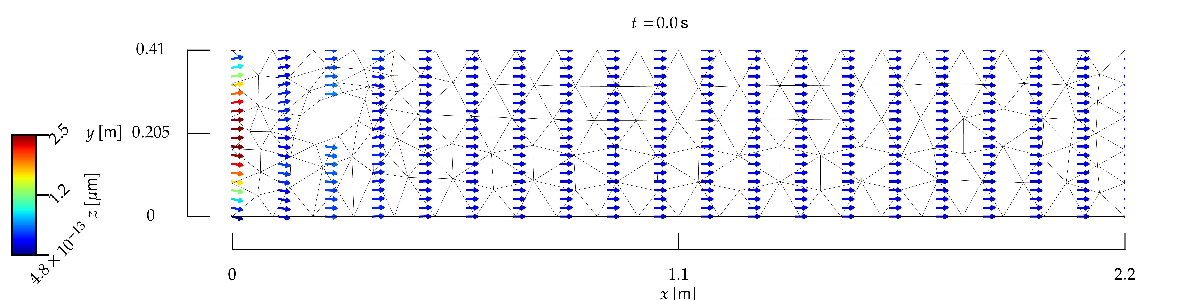
\includegraphics[width=1.05\columnwidth]{figures/figure_1/figure_1.pdf}
    \caption{
        \label{fig_no_circle}
        Curvature of the \Acl{mem}  interacting  with a \acl{bflu} shown in \cref{fig_fluid_mem}. The Figure follows the same notation and it corresponds to the same instant of time as \cref{fig_fluid_mem}.
    }
\end{figure}